\documentclass[conference]{IEEEtran}
\usepackage[utf8]{inputenc}
\usepackage[T1]{fontenc}
\usepackage[turkish]{babel}
\usepackage{amsmath,amssymb,amsfonts}
\usepackage{graphicx}
\usepackage{textcomp}
\usepackage{xcolor}
\usepackage{booktabs}
\usepackage{multirow}
\usepackage{hyperref}
\usepackage{float}
\usepackage{enumitem}
\usepackage{subcaption}
\usepackage{array}
\usepackage{tabularx}
\usepackage{cite}

\hypersetup{
    colorlinks=true,
    linkcolor=blue,
    citecolor=blue,
    urlcolor=blue
}

\graphicspath{{figures/}}

\begin{document}

\title{Yelp Restoran Yorumlarından Metin Madenciliği ile Kalite Tahmini: Klasik Makine Öğrenmesi ve Derin Öğrenme Yaklaşımlarının Karşılaştırmalı Analizi}

\author{
\IEEEauthorblockN{Taha Yasin Çiçek}
\IEEEauthorblockA{
Bilgisayar Mühendisliği Bölümü\\
Kocaeli Üniversitesi\\
Kocaeli, Türkiye\\
}
}

\maketitle

\begin{abstract}
Bu çalışmada, Yelp açık veri setinden elde edilen yaklaşık 1,6 milyon restoran yorumu üzerinde metin madenciliği teknikleri kullanılarak müşteri deneyimlerinin kalite sınıflandırması gerçekleştirilmiştir. Ham metin verileri kapsamlı bir doğal dil işleme (NLP) boru hattından geçirilerek TF-IDF ve dizi (sequence) tabanlı öznitelik vektörlerine dönüştürülmüştür. Lojistik Regresyon, Destek Vektör Makineleri (SVM), LightGBM, SGD, TextCNN ve FastText olmak üzere altı farklı model mimarisi eğitilmiş ve karşılaştırılmıştır. Deneysel sonuçlar, Lojistik Regresyon modelinin \%80,39 doğruluk ve \%80,38 F1-Makro skoru ile en yüksek performansı sergilediğini göstermektedir. Ayrıca, Açıklanabilir Yapay Zekâ (LIME) yöntemiyle model kararları yorumlanmış ve Yön-Bazlı Duygu Analizi (ABSA) ile yemek, servis, ambiyans ve fiyat gibi spesifik boyutlarda duygu analizi gerçekleştirilmiştir. Sonuçlar, önceden eğitilmiş Transformer modelleri (BERT vb.) kullanılmadan, klasik NLP yöntemleriyle 3-sınıflı subjektif bir görevde yüksek başarı elde edilebileceğini ortaya koymaktadır.
\end{abstract}

\begin{IEEEkeywords}
Metin madenciliği, duygu analizi, doğal dil işleme, TF-IDF, derin öğrenme, LSTM, restoran yorumları, Yelp, makine öğrenmesi, yön-bazlı duygu analizi
\end{IEEEkeywords}

% ============================================================
\section{Giriş}
\label{sec:giris}

Günümüzde çevrimiçi platformlardaki kullanıcı yorumları, tüketici karar alma süreçlerinde kritik bir rol oynamaktadır. Özellikle restoran sektöründe, Yelp, Google Reviews ve TripAdvisor gibi platformlardaki milyonlarca yorum, hem tüketiciler hem de işletme sahipleri için değerli bilgiler barındırmaktadır \cite{liu2012sentiment}. Bu yorumların otomatik olarak analiz edilmesi ve sınıflandırılması, metin madenciliği ve doğal dil işleme (NLP) alanlarının önemli uygulama alanlarından birini oluşturmaktadır.

Duygu analizi (sentiment analysis), metinlerdeki öznel bilgileri tespit etmeyi amaçlayan bir NLP alt alanıdır \cite{pang2008opinion}. Restoran yorumları bağlamında duygu analizi, yalnızca genel memnuniyet düzeyinin belirlenmesiyle sınırlı kalmayıp, yemek kalitesi, servis hızı, ambiyans ve fiyat gibi spesifik boyutlarda da değerlendirme yapılmasını mümkün kılmaktadır \cite{pontiki2016semeval}.

Bu çalışmanın temel katkıları şu şekilde özetlenebilir:
\begin{itemize}
    \item Yaklaşık 1,6 milyon Yelp restoran yorumu üzerinde kapsamlı bir metin madenciliği boru hattı tasarlanmış ve uygulanmıştır.
    \item Klasik makine öğrenmesi (Lojistik Regresyon, SVM, LightGBM, SGD) ve derin öğrenme (TextCNN, FastText) modelleri sistematik olarak karşılaştırılmıştır.
    \item LIME tabanlı açıklanabilir yapay zekâ yöntemiyle model kararları yorumlanmıştır.
    \item Yön-Bazlı Duygu Analizi (ABSA) ile restoran deneyiminin farklı boyutları ayrıştırılmıştır.
    \item Etkileşimli bir Flask web uygulaması geliştirilmiştir.
\end{itemize}

Makalenin geri kalanı şu şekilde düzenlenmiştir: Bölüm~\ref{sec:ilgili} ilgili çalışmaları, Bölüm~\ref{sec:veriset} veri setini, Bölüm~\ref{sec:yontem} önerilen yöntemi, Bölüm~\ref{sec:deneysel} deneysel sonuçları, Bölüm~\ref{sec:tartisma} tartışmayı ve Bölüm~\ref{sec:sonuc} sonuçları sunmaktadır.

% ============================================================
\section{İlgili Çalışmalar}
\label{sec:ilgili}

Restoran yorumlarından duygu analizi üzerine literatürde çok sayıda çalışma bulunmaktadır. Pang ve Lee \cite{pang2002thumbs}, film yorumları üzerinde Naive Bayes, Maksimum Entropi ve SVM sınıflandırıcılarını karşılaştırarak metin tabanlı duygu sınıflandırmasının temellerini atmıştır. 

TF-IDF (Term Frequency-Inverse Document Frequency) öznitelik çıkarımı, metin sınıflandırma görevlerinde yaygın olarak kullanılmaktadır \cite{salton1988term}. Bu yöntem, bir kelimenin bir belgede ne kadar önemli olduğunu, hem belge içi frekansını hem de külliyat genelindeki nadir görülme oranını dikkate alarak hesaplamaktadır.

Derin öğrenme yaklaşımları açısından, Kim \cite{kim2014convolutional} Evrişimli Sinir Ağlarını (CNN) metin sınıflandırma için uyarlayarak TextCNN mimarisini önermiştir. Hochreiter ve Schmidhuber \cite{hochreiter1997long} tarafından geliştirilen LSTM ağları ise sıralı verilerdeki uzun vadeli bağımlılıkları yakalamada başarılı olmuştur.

Joulin ve ark. \cite{joulin2017bag} tarafından önerilen FastText modeli, kelime n-gram'larını kullanarak hızlı ve etkili metin sınıflandırması yapmaktadır. Yön-bazlı duygu analizi (ABSA) konusunda ise SemEval yarışmaları \cite{pontiki2016semeval} bu alandaki araştırmaları önemli ölçüde teşvik etmiştir.

Açıklanabilir yapay zekâ (XAI) alanında, Ribeiro ve ark. \cite{ribeiro2016why} tarafından önerilen LIME (Local Interpretable Model-agnostic Explanations), herhangi bir sınıflandırıcının bireysel tahminlerini yorumlamak için kullanılan model-bağımsız bir yöntemdir.

% ============================================================
\section{Veri Seti}
\label{sec:veriset}

\subsection{Yelp Açık Veri Seti}
Bu çalışmada, Yelp tarafından akademik amaçlı sunulan açık veri seti (Yelp Open Dataset) kullanılmıştır. Ham veri seti, çeşitli iş kollarına ait milyonlarca yorum içermektedir. Çalışmamızda yalnızca restoran kategorisine ait işletmelerin yorumları filtrelenmiştir.

\subsection{Veri Filtreleme ve Temizleme}
Veri hazırlama süreci aşağıdaki adımlardan oluşmaktadır:

\begin{enumerate}
    \item \textbf{İşletme Filtreleme:} \texttt{yelp\_academic\_dataset\_business.json} dosyasından ``Restaurants'' kategorisini içeren 52.268 işletme tespit edilmiştir.
    \item \textbf{Yorum Filtreleme:} Bu işletmelere ait toplam 4.724.471 yorum çıkarılmıştır.
    \item \textbf{Veri Temizliği:} Boş, 10 karakterden kısa ve tekrarlanan yorumlar çıkarılmış, 4.724.364 yorum kalmıştır.
    \item \textbf{Sınıf Dönüşümü:} 5 yıldızlı puanlama sistemi 3 sınıfa dönüştürülmüştür:
    \begin{itemize}
        \item 1-2 yıldız $\rightarrow$ \textbf{Kötü} (Sınıf 0)
        \item 3 yıldız $\rightarrow$ \textbf{Orta} (Sınıf 1)
        \item 4-5 yıldız $\rightarrow$ \textbf{İyi} (Sınıf 2)
    \end{itemize}
    \item \textbf{Sınıf Dengeleme:} Orijinal dağılımda İyi sınıfı \%67,94, Kötü \%20,57 ve Orta \%11,50 oranındadır. Azınlık sınıfı olan Orta'nın örnek sayısı (543.093) baz alınarak alt-örnekleme (undersampling) uygulanmış ve her sınıftan eşit sayıda örnek seçilmiştir.
\end{enumerate}

Sonuç olarak, dengeli veri seti toplamda \textbf{1.629.279 yorum} içermektedir (her sınıfta 543.093 örnek).

\begin{figure}[htbp]
    \centering
    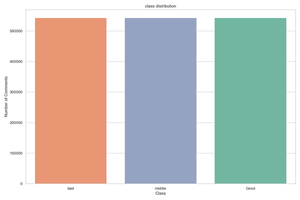
\includegraphics[width=3cm]{eda_class_distribution.png}
    \caption{Dengeleme sonrası sınıf dağılımı.}
    \label{fig:sinif_dagilim}
\end{figure}

% ============================================================
\section{Önerilen Yöntem}
\label{sec:yontem}

Önerilen yöntem, Şekil~\ref{fig:pipeline}'de gösterildiği gibi birbirini takip eden yedi aşamadan oluşan modüler bir boru hattı şeklinde tasarlanmıştır.

\begin{figure}[htbp]
    \centering
    \fbox{\parbox{0.9\columnwidth}{
    \centering
    \small
    \textbf{1. Veri Hazırlama} $\downarrow$ \\
    \textbf{2. Keşifsel Veri Analizi (EDA)} $\downarrow$ \\
    \textbf{3. Metin Ön İşleme} $\downarrow$ \\
    \textbf{4. Öznitelik Çıkarımı} $\downarrow$ \\
    \textbf{5. Model Eğitimi} $\downarrow$ \\
    \textbf{6. Model Değerlendirme} $\downarrow$ \\
    \textbf{7. Yön-Bazlı Duygu Analizi}
    }}
    \caption{Önerilen boru hattı mimarisi.}
    \label{fig:pipeline}
\end{figure}

\subsection{Keşifsel Veri Analizi (EDA)}

Veri setinin temel özelliklerini anlamak amacıyla kapsamlı bir keşifsel veri analizi gerçekleştirilmiştir. Yorum uzunlukları, kelime sayıları, yıldız dağılımları, zaman trendleri ve sosyal etkileşim metrikleri (useful, funny, cool) incelenmiştir. Her sınıf için kelime bulutu (word cloud) ve n-gram analizleri yapılmıştır.

\begin{figure}[htbp]
    \centering
    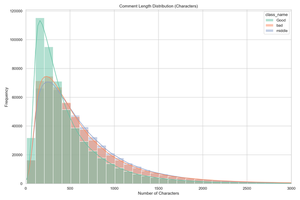
\includegraphics[width=3cm]{eda_review_length.png}
    \caption{Sınıflara göre yorum uzunluğu dağılımı.}
    \label{fig:yorum_uzunluk}
\end{figure}

\begin{figure}[htbp]
    \centering
    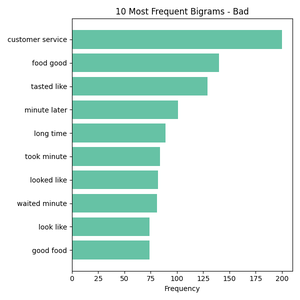
\includegraphics[width=3cm]{eda_bigrams_bad.png}
    \caption{En sık kullanılan ikili kelimeler - Kötü Sınıf}
    \label{fig:bigrams_bad}
\end{figure}

\begin{figure}[htbp]
    \centering
    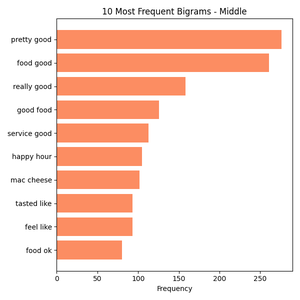
\includegraphics[width=3cm]{eda_bigrams_middle.png}
    \caption{En sık kullanılan ikili kelimeler - Orta Sınıf}
    \label{fig:bigrams_middle}
\end{figure}

\begin{figure}[htbp]
    \centering
    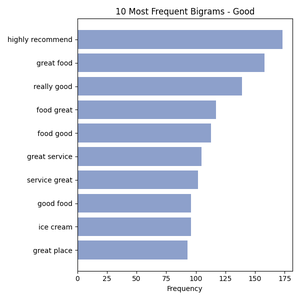
\includegraphics[width=3cm]{eda_bigrams_good.png}
    \caption{En sık kullanılan ikili kelimeler - İyi Sınıf}
    \label{fig:bigrams_good}
\end{figure}

Analiz sonuçlarına göre, olumsuz (Kötü) sınıftaki yorumlar ortalama 655 karakter uzunluğunda iken, olumlu (İyi) sınıftaki yorumlar ortalama 492 karakter ile daha kısa olma eğilimindedir. Bu bulgu, memnuniyetsiz müşterilerin deneyimlerini daha detaylı anlatma eğiliminde olduğunu göstermektedir.

\subsection{Metin Ön İşleme}

Metin ön işleme aşaması aşağıdaki adımlardan oluşmaktadır:

\begin{enumerate}
    \item Küçük harfe dönüştürme
    \item HTML etiketleri ve URL'lerin temizlenmesi
    \item Emoji ve Unicode karakterlerin kaldırılması
    \item Noktalama işaretleri ve özel karakterlerin çıkarılması
    \item Sayısal değerlerin kaldırılması
    \item Fazla boşlukların temizlenmesi
    \item Tokenizasyon (NLTK \texttt{word\_tokenize})
    \item Durak kelime (stopword) çıkarımı — olumsuzluk kelimeleri korunarak
    \item WordNet Lemmatizasyonu
    \item 2 karakterden kısa kelimelerin çıkarılması
\end{enumerate}

Durak kelime çıkarımında, duygu analizinde kritik öneme sahip olumsuzluk kelimeleri (\textit{not, no, nor, don't, isn't, wouldn't} vb.) korunmuştur. Bu yaklaşım, ``the food is \textit{not} good'' gibi cümlelerin anlam bütünlüğünü korumak açısından önemlidir.

\subsubsection{Ek Öznitelik Mühendisliği}
Ham metin özniteliklerine ek olarak, Tablo~\ref{tab:ozellikler}'de listelenen sayısal öznitelikler çıkarılmıştır.

\begin{table}[htbp]
\centering
\caption{Çıkarılan sayısal öznitelikler ve sınıf bazlı ortalamaları.}
\label{tab:ozellikler}
\small
\begin{tabular}{lrrr}
\toprule
\textbf{Öznitelik} & \textbf{Kötü} & \textbf{Orta} & \textbf{İyi} \\
\midrule
Yorum Uzunluğu (karakter) & 655,50 & 659,26 & 491,78 \\
Kelime Sayısı & 122,42 & 122,23 & 89,82 \\
Ünlem Sayısı & 0,86 & 0,58 & 1,56 \\
Soru İşareti Sayısı & 0,34 & 0,21 & 0,10 \\
Ort. Kelime Uzunluğu & 4,39 & 4,41 & 4,54 \\
Büyük Harf Oranı & 0,027 & 0,025 & 0,030 \\
TextBlob Polarite & $-0,007$ & 0,185 & 0,351 \\
TextBlob Subjektivite & 0,530 & 0,548 & 0,592 \\
\bottomrule
\end{tabular}
\end{table}

TextBlob kütüphanesi kullanılarak hesaplanan duygu polaritesi, sınıflar arasında belirgin farklılıklar göstermektedir: Kötü sınıfı neredeyse nötr ($-0,007$), Orta sınıfı hafif pozitif ($0,185$) ve İyi sınıfı güçlü pozitif ($0,351$) polariteye sahiptir.

\begin{figure}[htbp]
    \centering
    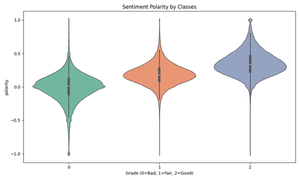
\includegraphics[width=3cm]{preprocessing_features.png}
    \caption{Sınıflara göre TextBlob duygu polaritesi dağılımı (keman grafiği).}
    \label{fig:polarity}
\end{figure}

\subsection{Öznitelik Çıkarımı}

İki farklı öznitelik temsili oluşturulmuştur:

\subsubsection{TF-IDF Vektörizasyonu}
Klasik makine öğrenmesi modelleri için TF-IDF (Term Frequency–Inverse Document Frequency) yöntemi kullanılmıştır. Parametreler: \texttt{max\_features=50000}, \texttt{ngram\_range=(1,2)}, \texttt{sublinear\_tf=True}, \texttt{min\_df=2}, \texttt{max\_df=0.95}. TF-IDF matrisi, StandardScaler ile normalize edilmiş 8 sayısal öznitelikle birleştirilerek $(1.629.206 \times 50.008)$ boyutunda bir birleşik öznitelik matrisi elde edilmiştir.

\subsubsection{Dizi Kodlama (Sequence Encoding)}
Derin öğrenme modelleri için Keras \texttt{Tokenizer} kullanılmıştır. En sık 50.000 kelime seçilmiş, her yorum 200 token uzunluğunda sabitlenmiştir (kısa yorumlar sıfırla doldurulmuş, uzun yorumlar kesilmiştir). Toplam sözlük büyüklüğü 222.483 benzersiz kelimedir.

\subsection{Veri Bölütleme}
Veri seti tabakalı örnekleme (stratified sampling) ile üç parçaya ayrılmıştır:
\begin{itemize}
    \item \textbf{Eğitim:} 1.140.444 örnek (\%70)
    \item \textbf{Doğrulama:} 244.381 örnek (\%15)
    \item \textbf{Test:} 244.381 örnek (\%15)
\end{itemize}
Her alt kümede sınıf dağılımı eşit (\%33,3) tutulmuştur.

\subsection{Model Mimarileri}

\subsubsection{Lojistik Regresyon (LR)}
TF-IDF + sayısal öznitelikler üzerinde eğitilmiştir. \texttt{max\_iter=2000}, \texttt{solver=`lbfgs'}, çok sınıflı strateji olarak \texttt{multi\_class=`multinomial'} kullanılmıştır. Tüm eğitim verisi (1.140.444 örnek) ile eğitilmiştir.

\subsubsection{Destek Vektör Makineleri (SVM)}
\texttt{LinearSVC} sınıflandırıcısı, \texttt{CalibratedClassifierCV} sarmalayıcısı ile olasılık tahmini yapabilir hâle getirilmiştir. TF-IDF + sayısal öznitelikler üzerinde tüm eğitim verisiyle eğitilmiştir.

\subsubsection{LightGBM}
Gradyan artırma (gradient boosting) çerçevesi olan LightGBM, TF-IDF öznitelikleri üzerinde eğitilmiştir. Büyük ve seyrek matrislerle verimli çalışabilme avantajı sunan bu model, tüm eğitim verisiyle eğitilmiştir.

\subsubsection{TextCNN}
Kim \cite{kim2014convolutional}'in önerdiği CNN tabanlı metin sınıflandırma mimarisi uyarlanmıştır. 128 boyutlu gömme (embedding) katmanı, çoklu filtre boyutlarına sahip evrişim katmanları, global max pooling ve yoğun (dense) katmanlardan oluşmaktadır. CPU kısıtları nedeniyle 25.000 örneklik alt küme üzerinde eğitilmiştir.

\subsubsection{FastText}
Joulin ve ark. \cite{joulin2017bag}'nın yaklaşımından esinlenerek tasarlanmıştır. 128 boyutlu gömme katmanı, \texttt{GlobalAveragePooling1D}, 64 birimlik yoğun katman, \%30 Dropout ve softmax çıkış katmanından oluşmaktadır. Eğitim süresi yalnızca 12 saniyedir.

\subsubsection{SGD Sınıflandırıcı}
Stokastik Gradyan İnişi (SGD) tabanlı doğrusal sınıflandırıcı, log-loss kaybı ve dengeli sınıf ağırlıkları ile TF-IDF matrisi üzerinde eğitilmiştir.

% ============================================================
\section{Deneysel Sonuçlar}
\label{sec:deneysel}

\subsection{Değerlendirme Metrikleri}
Model performansları aşağıdaki metriklerle değerlendirilmiştir:

\begin{itemize}
    \item \textbf{Doğruluk (Accuracy):} Doğru tahminlerin toplam tahminlere oranı.
    \item \textbf{Kesinlik (Precision):} Pozitif olarak tahmin edilenlerin gerçekten pozitif olma oranı.
    \item \textbf{Duyarlılık (Recall):} Gerçek pozitiflerin doğru tahmin edilme oranı.
    \item \textbf{F1-Makro Skoru:} Her sınıf için hesaplanan F1 skorlarının aritmetik ortalaması.
\end{itemize}

\subsection{Test Seti Sonuçları}

Tablo~\ref{tab:test_sonuc}'da tüm modellerin test seti üzerindeki performansları sunulmaktadır.

\begin{table}[htbp]
\centering
\caption{Modellerin test seti üzerindeki performans karşılaştırması.}
\label{tab:test_sonuc}
\small
\begin{tabular}{lcccc}
\toprule
\textbf{Model} & \textbf{Doğr.} & \textbf{Kes.} & \textbf{Duy.} & \textbf{F1-M} \\
\midrule
\textbf{Lojistik Reg.} & \textbf{0,8039} & \textbf{0,8038} & \textbf{0,8039} & \textbf{0,8038} \\
SVM & 0,8012 & 0,7996 & 0,8012 & 0,8002 \\
FastText & 0,7562 & 0,7527 & 0,7562 & 0,7538 \\
SGD & 0,7552 & 0,7523 & 0,7552 & 0,7530 \\
TextCNN & 0,7481 & 0,7502 & 0,7481 & 0,7490 \\
\bottomrule
\end{tabular}
\end{table}

\begin{table}[htbp]
\centering
\caption{Doğrulama seti üzerindeki ek model performansları.}
\label{tab:val_sonuc}
\small
\begin{tabular}{lccc}
\toprule
\textbf{Model} & \textbf{Doğruluk} & \textbf{F1-Makro} & \textbf{Veri Boyutu} \\
\midrule
Lojistik Reg. & 0,7979 & 0,7978 & Tam (1,14M) \\
SVM & 0,7950 & 0,7940 & Tam (1,14M) \\
LightGBM & 0,7923 & 0,7925 & Tam (1,14M) \\
BiLSTM & 0,7432 & 0,7443 & Alt küme (25K) \\
LSTM & 0,3342 & 0,1719 & Alt küme (25K) \\
\bottomrule
\end{tabular}
\end{table}

Sonuçlar incelendiğinde, TF-IDF tabanlı klasik modellerin (LR, SVM, LightGBM) derin öğrenme modellerinden (TextCNN, FastText, BiLSTM) tutarlı bir şekilde daha iyi performans sergilediği görülmektedir. Bu durum, büyük ölçekli eğitim verisi avantajının ve TF-IDF'in 50.000 öznitelikli zengin temsilinin etkisiyle açıklanabilir.

\subsection{Karışıklık Matrisleri}

\begin{figure}[htbp]
    \centering
    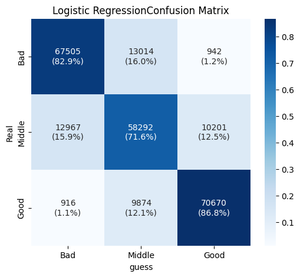
\includegraphics[width=3cm]{confusion_matrix_Logistic_Regression.png}
    \caption{Karışıklık Matrisi - Lojistik Regresyon}
    \label{fig:cm_lr}
\end{figure}

\begin{figure}[htbp]
    \centering
    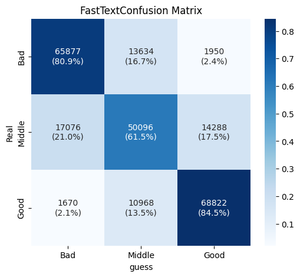
\includegraphics[width=3cm]{confusion_matrix_FastText.png}
    \caption{Karışıklık Matrisi - FastText}
    \label{fig:cm_ft}
\end{figure}

Karışıklık matrisleri (Şekil~\ref{fig:confusion}) incelendiğinde, tüm modellerde en yaygın hatanın ``Kötü'' ve ``Orta'' sınıfları arasındaki karışıklık olduğu gözlemlenmektedir. Bu durum, 2-3 yıldızlı yorumların dilsel olarak birbirine yakın olmasından kaynaklanmaktadır. ``İyi'' sınıfı ise tüm modellerde en yüksek doğrulukla sınıflandırılmaktadır.

\subsection{ROC ve Precision-Recall Eğrileri}

\begin{figure}[htbp]
    \centering
    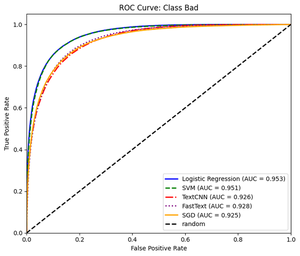
\includegraphics[width=3cm]{roc_curve_class_Bad.png}
    \caption{ROC Eğrisi - Kötü Sınıf}
    \label{fig:roc_bad}
\end{figure}

\begin{figure}[htbp]
    \centering
    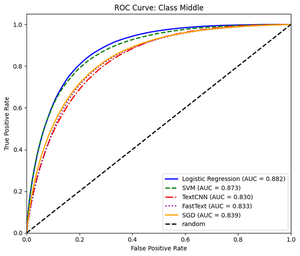
\includegraphics[width=3cm]{roc_curve_class_Middle.png}
    \caption{ROC Eğrisi - Orta Sınıf}
    \label{fig:roc_middle}
\end{figure}

\begin{figure}[htbp]
    \centering
    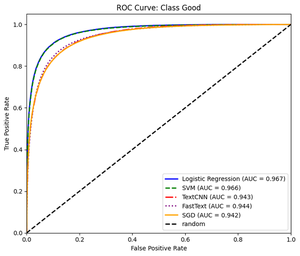
\includegraphics[width=3cm]{roc_curve_class_Good.png}
    \caption{ROC Eğrisi - İyi Sınıf}
    \label{fig:roc_good}
\end{figure}

\begin{figure}[htbp]
    \centering
    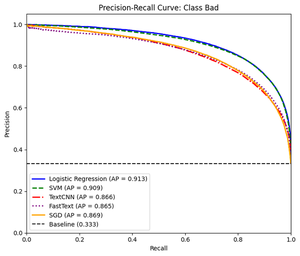
\includegraphics[width=3cm]{pr_curve_class_Bad.png}
    \caption{Precision-Recall Eğrisi - Kötü Sınıf}
    \label{fig:pr_bad}
\end{figure}

\begin{figure}[htbp]
    \centering
    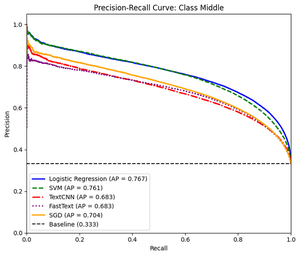
\includegraphics[width=3cm]{pr_curve_class_Middle.png}
    \caption{Precision-Recall Eğrisi - Orta Sınıf}
    \label{fig:pr_middle}
\end{figure}

\begin{figure}[htbp]
    \centering
    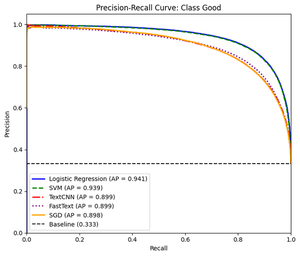
\includegraphics[width=3cm]{pr_curve_class_Good.png}
    \caption{Precision-Recall Eğrisi - İyi Sınıf}
    \label{fig:pr_good}
\end{figure}

ROC eğrileri (Şekil~\ref{fig:roc}) ve Precision-Recall eğrileri (Şekil~\ref{fig:pr}), Lojistik Regresyon ve SVM modellerinin tüm sınıflarda yüksek AUC değerlerine sahip olduğunu doğrulamaktadır.

\subsection{Radar Grafik Karşılaştırması}

\begin{figure}[htbp]
    \centering
    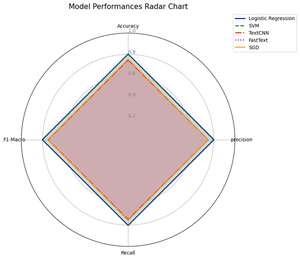
\includegraphics[width=3cm]{model_comparison_radar.png}
    \caption{Modellerin çoklu metrik radar grafiği karşılaştırması.}
    \label{fig:radar}
\end{figure}

Radar grafiği (Şekil~\ref{fig:radar}), modellerin dört farklı metrik (Doğruluk, Kesinlik, Duyarlılık, F1-Makro) üzerindeki performanslarını görsel olarak karşılaştırmaktadır. Lojistik Regresyon ve SVM'in tüm metriklerde benzer ve yüksek performans sergilediği açıkça görülmektedir.

\subsection{Eğitim Süreçleri Analizi}

\begin{figure}[htbp]
    \centering
    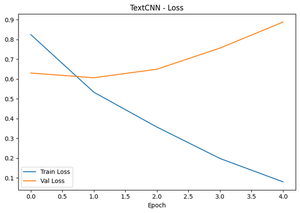
\includegraphics[width=3cm]{training_history_cnn_loss.png}
    \caption{Eğitim Geçmişi - TextCNN Kayıp (Loss)}
    \label{fig:hist_cnn_loss}
\end{figure}

\begin{figure}[htbp]
    \centering
    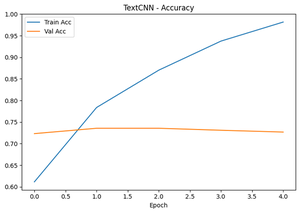
\includegraphics[width=3cm]{training_history_cnn_accuracy.png}
    \caption{Eğitim Geçmişi - TextCNN Doğruluk (Acc)}
    \label{fig:hist_cnn_acc}
\end{figure}

\begin{figure}[htbp]
    \centering
    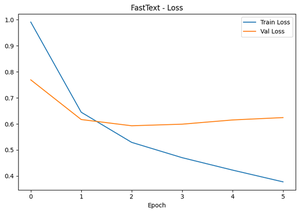
\includegraphics[width=3cm]{training_history_fasttext_loss.png}
    \caption{Eğitim Geçmişi - FastText Kayıp (Loss)}
    \label{fig:hist_ft_loss}
\end{figure}

\begin{figure}[htbp]
    \centering
    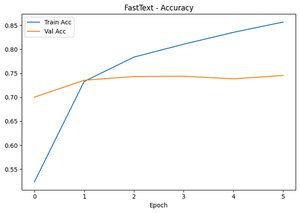
\includegraphics[width=3cm]{training_history_fasttext_accuracy.png}
    \caption{Eğitim Geçmişi - FastText Doğruluk (Acc)}
    \label{fig:hist_ft_acc}
\end{figure}

Derin öğrenme modellerinin eğitim geçmişleri (Şekil~\ref{fig:training}), EarlyStopping mekanizması sayesinde aşırı öğrenmenin (overfitting) kontrol altında tutulduğunu göstermektedir.

\subsection{Hata Analizi}

En iyi performans gösteren model (Lojistik Regresyon) üzerinde detaylı hata analizi gerçekleştirilmiştir. Toplam 244.381 test örneğinden 47.914'ü (\%19,61) yanlış sınıflandırılmıştır.

\begin{figure}[htbp]
    \centering
    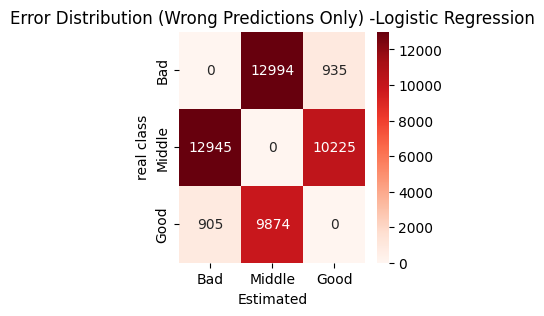
\includegraphics[width=3cm]{error_analysis.png}
    \caption{En iyi modelin (LR) hata dağılımı matrisi.}
    \label{fig:error}
\end{figure}

Hata analizi sonuçları (Şekil~\ref{fig:error}), yanlış tahminlerin büyük çoğunluğunun komşu sınıflar arasında gerçekleştiğini ortaya koymaktadır. Bu, 3 sınıflı duygu analizi görevlerinde beklenen bir durumdur; zira ``Kötü'' ile ``Orta'' veya ``Orta'' ile ``İyi'' arasındaki dilsel sınır çoğu zaman belirsizdir.

\subsection{Açıklanabilir Yapay Zekâ (LIME)}

Model kararlarının şeffaflığını sağlamak amacıyla LIME yöntemi uygulanmıştır. LIME, bireysel tahminleri açıklamak için orijinal metindeki kelimeleri perturbe ederek her kelimenin tahmine olan katkısını hesaplamaktadır.

Örnek bir analiz sonucunda, ``best'', ``perfect'', ``excellent'' gibi kelimelerin ``İyi'' sınıfına güçlü pozitif katkı sağladığı; ``terrible'', ``worst'', ``disgusting'' gibi kelimelerin ise ``Kötü'' sınıfına yönlendirdiği tespit edilmiştir. LIME sonuçları, modelin semantik olarak anlamlı kelime-duygu ilişkilerini öğrendiğini doğrulamaktadır.

\subsection{Yön-Bazlı Duygu Analizi (ABSA)}

Genel duygu sınıflandırmasının ötesinde, her yorumun cümle düzeyinde ayrıştırılarak belirli restoran boyutları (yönler) açısından analiz edilmesi gerçekleştirilmiştir. Tanımlanan yönler ve ilişkili anahtar kelimeler Tablo~\ref{tab:aspect}'te sunulmaktadır.

\begin{table}[htbp]
\centering
\caption{Yön-Bazlı Duygu Analizi için tanımlanan yönler ve anahtar kelimeler.}
\label{tab:aspect}
\small
\begin{tabular}{lp{5cm}}
\toprule
\textbf{Yön} & \textbf{Anahtar Kelimeler} \\
\midrule
Yemek & food, meal, delicious, taste, chicken, burger, pizza, fresh, flavor \\
Servis & service, waiter, staff, manager, rude, friendly, slow, fast \\
Ambiyans & place, atmosphere, vibe, clean, dirty, loud, quiet, music, decor \\
Fiyat & price, cost, expensive, cheap, worth, value, bill, money \\
\bottomrule
\end{tabular}
\end{table}

\begin{figure}[htbp]
    \centering
    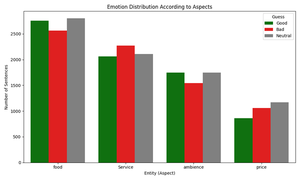
\includegraphics[width=3cm]{aspect_based_sentiment.png}
    \caption{Yön-bazlı duygu analizi sonuçları.}
    \label{fig:absa}
\end{figure}

10.000 örneklik bir alt kümede gerçekleştirilen ABSA analizinde toplam 22.710 yön-cümle eşleşmesi tespit edilmiştir (Şekil~\ref{fig:absa}). Yemek ve ambiyans yönlerinde olumlu duyguların ağırlıklı olduğu, servis yönünde ise olumsuz duyguların nispeten daha fazla olduğu gözlemlenmiştir.

% ============================================================
\section{Web Uygulaması}
\label{sec:webapp}

Projenin uygulamaya dönük boyutu olarak Flask tabanlı etkileşimli bir web uygulaması geliştirilmiştir. Uygulama üç temel işlev sunmaktadır:

\begin{enumerate}
    \item \textbf{Gerçek Zamanlı Tahmin:} Kullanıcı tarafından girilen metin, birden fazla model (LightGBM, SVM, LR) tarafından eş zamanlı olarak sınıflandırılmaktadır.
    \item \textbf{Toplu Analiz:} CSV formatında yüklenen yorum dosyaları toplu olarak analiz edilmekte ve duygu dağılımı grafikleri oluşturulmaktadır.
    \item \textbf{EDA Panoları:} Eğitim veri setine ait kelime bulutları, n-gram analizleri ve sınıf dağılımları etkileşimli grafiklerle görselleştirilmektedir.
\end{enumerate}

% ============================================================
\section{Tartışma}
\label{sec:tartisma}

\subsection{Klasik Modeller vs. Derin Öğrenme}
Deneysel sonuçlar, TF-IDF tabanlı klasik modellerin (LR: \%80,39, SVM: \%80,12) derin öğrenme modellerinden (FastText: \%75,62, TextCNN: \%74,81) tutarlı bir şekilde daha iyi performans sergilediğini göstermektedir. Bu sonuç, aşağıdaki faktörlerle açıklanabilir:

\begin{itemize}
    \item \textbf{Eğitim verisi büyüklüğü:} Klasik modeller tüm eğitim verisiyle (1,14M örnek) eğitilirken, derin öğrenme modelleri CPU kısıtları nedeniyle yalnızca 25.000 örneklik alt kümelerle eğitilmiştir.
    \item \textbf{TF-IDF'in etkinliği:} Bigram (1,2) destekli 50.000 öznitelikli TF-IDF temsili, restoran yorumlarındaki ayırt edici kelime ve kelime çiftlerini etkili bir şekilde yakalamaktadır.
    \item \textbf{Görev karmaşıklığı:} 3 sınıflı duygu analizi, ikili (pozitif/negatif) sınıflandırmaya kıyasla daha zor bir görevdir. Özellikle ``Orta'' sınıfı, hem olumlu hem olumsuz ifadeler içerebilmektedir.
\end{itemize}

\subsection{LSTM Performansı}
LSTM modelinin son derece düşük performansı (\%33,42 doğruluk — rastgele tahmin seviyesi) dikkat çekicidir. Bu durum, yetersiz eğitim verisi, hiperparametre optimizasyonunun yapılmamış olması ve sınırlı eğitim epoch sayısıyla açıklanabilir. Buna karşın, BiLSTM modeli \%74,32 doğrulukla çift yönlü bağlam yakalama avantajını göstermiştir.

\subsection{Sınırlamalar ve Gelecek Çalışmalar}
\begin{itemize}
    \item Derin öğrenme modelleri GPU ile tam veri seti üzerinde eğitildiğinde performanslarının önemli ölçüde artması beklenmektedir.
    \item BERT, RoBERTa gibi önceden eğitilmiş Transformer modelleri, ince ayar (fine-tuning) ile daha yüksek doğruluk sağlayabilir.
    \item ABSA modülü, kural tabanlı yaklaşım yerine dizin tabanlı (sequence labeling) yöntemlerle geliştirilebilir.
    \item Çapraz dil desteği eklenerek farklı dillerdeki yorumlar da analiz edilebilir.
\end{itemize}

% ============================================================
\section{Sonuç}
\label{sec:sonuc}

Bu çalışmada, Yelp açık veri setinden elde edilen 1,6 milyon restoran yorumu üzerinde kapsamlı bir metin madenciliği ve duygu analizi sistemi tasarlanmış ve uygulanmıştır. Çalışmanın temel bulguları şu şekilde özetlenebilir:

\begin{enumerate}
    \item Lojistik Regresyon, TF-IDF öznitelikleriyle \%80,39 doğruluk ve \%80,38 F1-Makro skoru elde ederek en yüksek performansı sergilemiştir.
    \item Klasik makine öğrenmesi modelleri, sınırlı kaynaklarla eğitilen derin öğrenme modellerinden tutarlı bir şekilde üstün performans göstermiştir.
    \item TextBlob duygu polaritesi, sınıflar arası güçlü ayırt edicilik özelliği taşımaktadır.
    \item LIME analizi, modelin semantik olarak anlamlı kelime-duygu ilişkilerini öğrendiğini doğrulamıştır.
    \item ABSA ile restoran deneyiminin farklı boyutları başarılı bir şekilde ayrıştırılmıştır.
\end{enumerate}

Sonuç olarak, önceden eğitilmiş Transformer modelleri kullanılmadan, iyi tasarlanmış bir öznitelik mühendisliği boru hattı ve klasik makine öğrenmesi algoritmaları ile 3 sınıflı subjektif bir NLP görevinde \%80'in üzerinde başarı elde edilebileceği gösterilmiştir. Bu sonuç, kaynak kısıtlı ortamlarda klasik yaklaşımların hâlâ rekabetçi olduğunu ortaya koymaktadır.

% ============================================================
\begin{thebibliography}{99}

\bibitem{liu2012sentiment}
B. Liu, ``Sentiment analysis and opinion mining,'' \textit{Synthesis Lectures on Human Language Technologies}, vol. 5, no. 1, pp. 1--167, 2012.

\bibitem{pang2008opinion}
B. Pang and L. Lee, ``Opinion mining and sentiment analysis,'' \textit{Foundations and Trends in Information Retrieval}, vol. 2, no. 1--2, pp. 1--135, 2008.

\bibitem{pontiki2016semeval}
M. Pontiki, D. Galanis, H. Papageorgiou, I. Androutsopoulos, S. Manandhar, M. AL-Smadi, M. Al-Ayyoub, Y. Zhao, B. Qin, O. De Clercq, and others, ``SemEval-2016 task 5: Aspect based sentiment analysis,'' in \textit{Proc. 10th Int. Workshop Semantic Evaluation (SemEval-2016)}, 2016, pp. 19--30.

\bibitem{pang2002thumbs}
B. Pang, L. Lee, and S. Vaithyanathan, ``Thumbs up? Sentiment classification using machine learning techniques,'' in \textit{Proc. ACL-02 Conf. Empirical Methods in Natural Language Processing}, 2002, pp. 79--86.

\bibitem{salton1988term}
G. Salton and C. Buckley, ``Term-weighting approaches in automatic text retrieval,'' \textit{Information Processing \& Management}, vol. 24, no. 5, pp. 513--523, 1988.

\bibitem{kim2014convolutional}
Y. Kim, ``Convolutional neural networks for sentence classification,'' in \textit{Proc. 2014 Conf. Empirical Methods in Natural Language Processing (EMNLP)}, 2014, pp. 1746--1751.

\bibitem{hochreiter1997long}
S. Hochreiter and J. Schmidhuber, ``Long short-term memory,'' \textit{Neural Computation}, vol. 9, no. 8, pp. 1735--1780, 1997.

\bibitem{joulin2017bag}
A. Joulin, E. Grave, P. Bojanowski, and T. Mikolov, ``Bag of tricks for efficient text classification,'' in \textit{Proc. 15th Conf. European Chapter of the Association for Computational Linguistics (EACL)}, 2017, pp. 427--431.

\bibitem{ribeiro2016why}
M. T. Ribeiro, S. Singh, and C. Guestrin, ``Why should I trust you? Explaining the predictions of any classifier,'' in \textit{Proc. 22nd ACM SIGKDD Int. Conf. Knowledge Discovery and Data Mining}, 2016, pp. 1135--1144.

\end{thebibliography}

\end{document}
